%\section{Protocols}
%\subsection{TCP vs. UDP}
\begin{frame}{TCP vs. UDP}{}
	\begin{center} 
		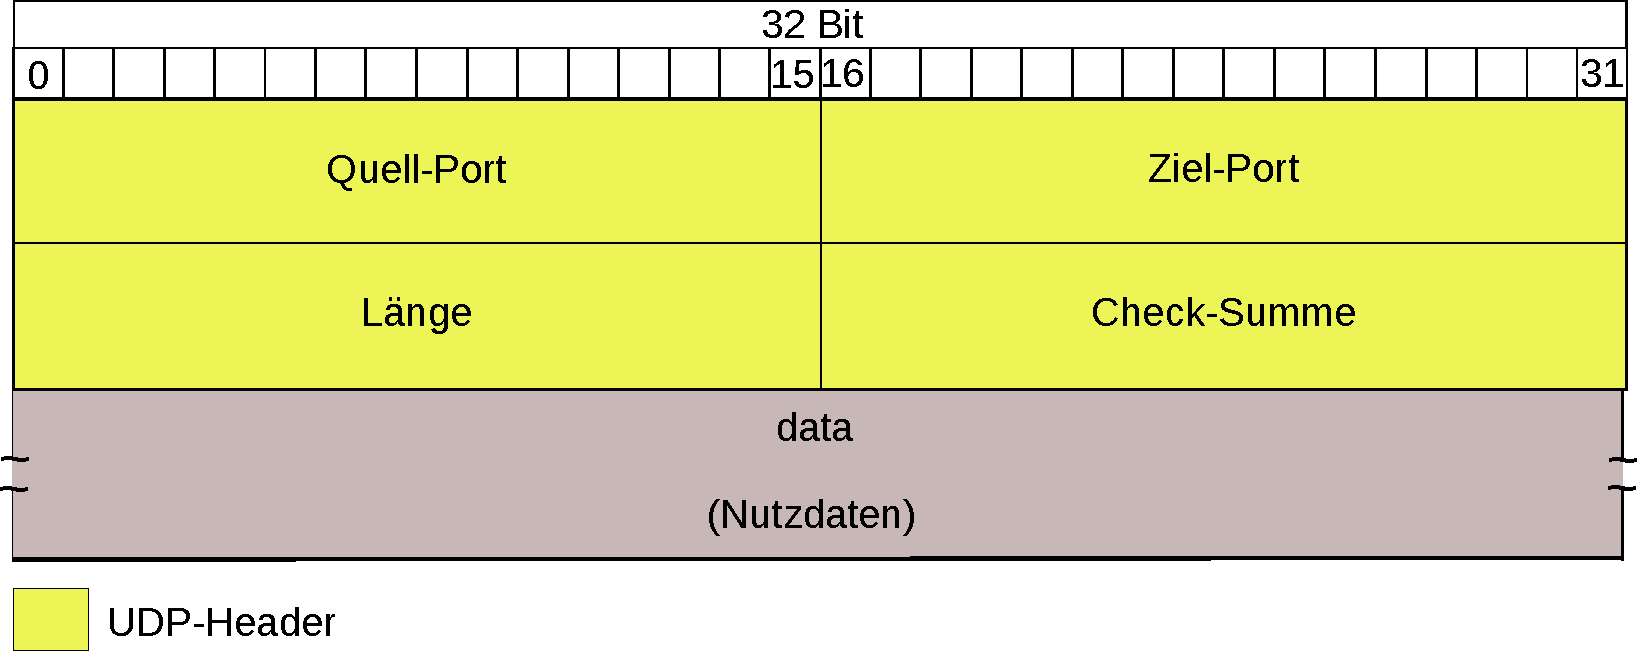
\includegraphics[width=0.5\textwidth]{udpheader}
		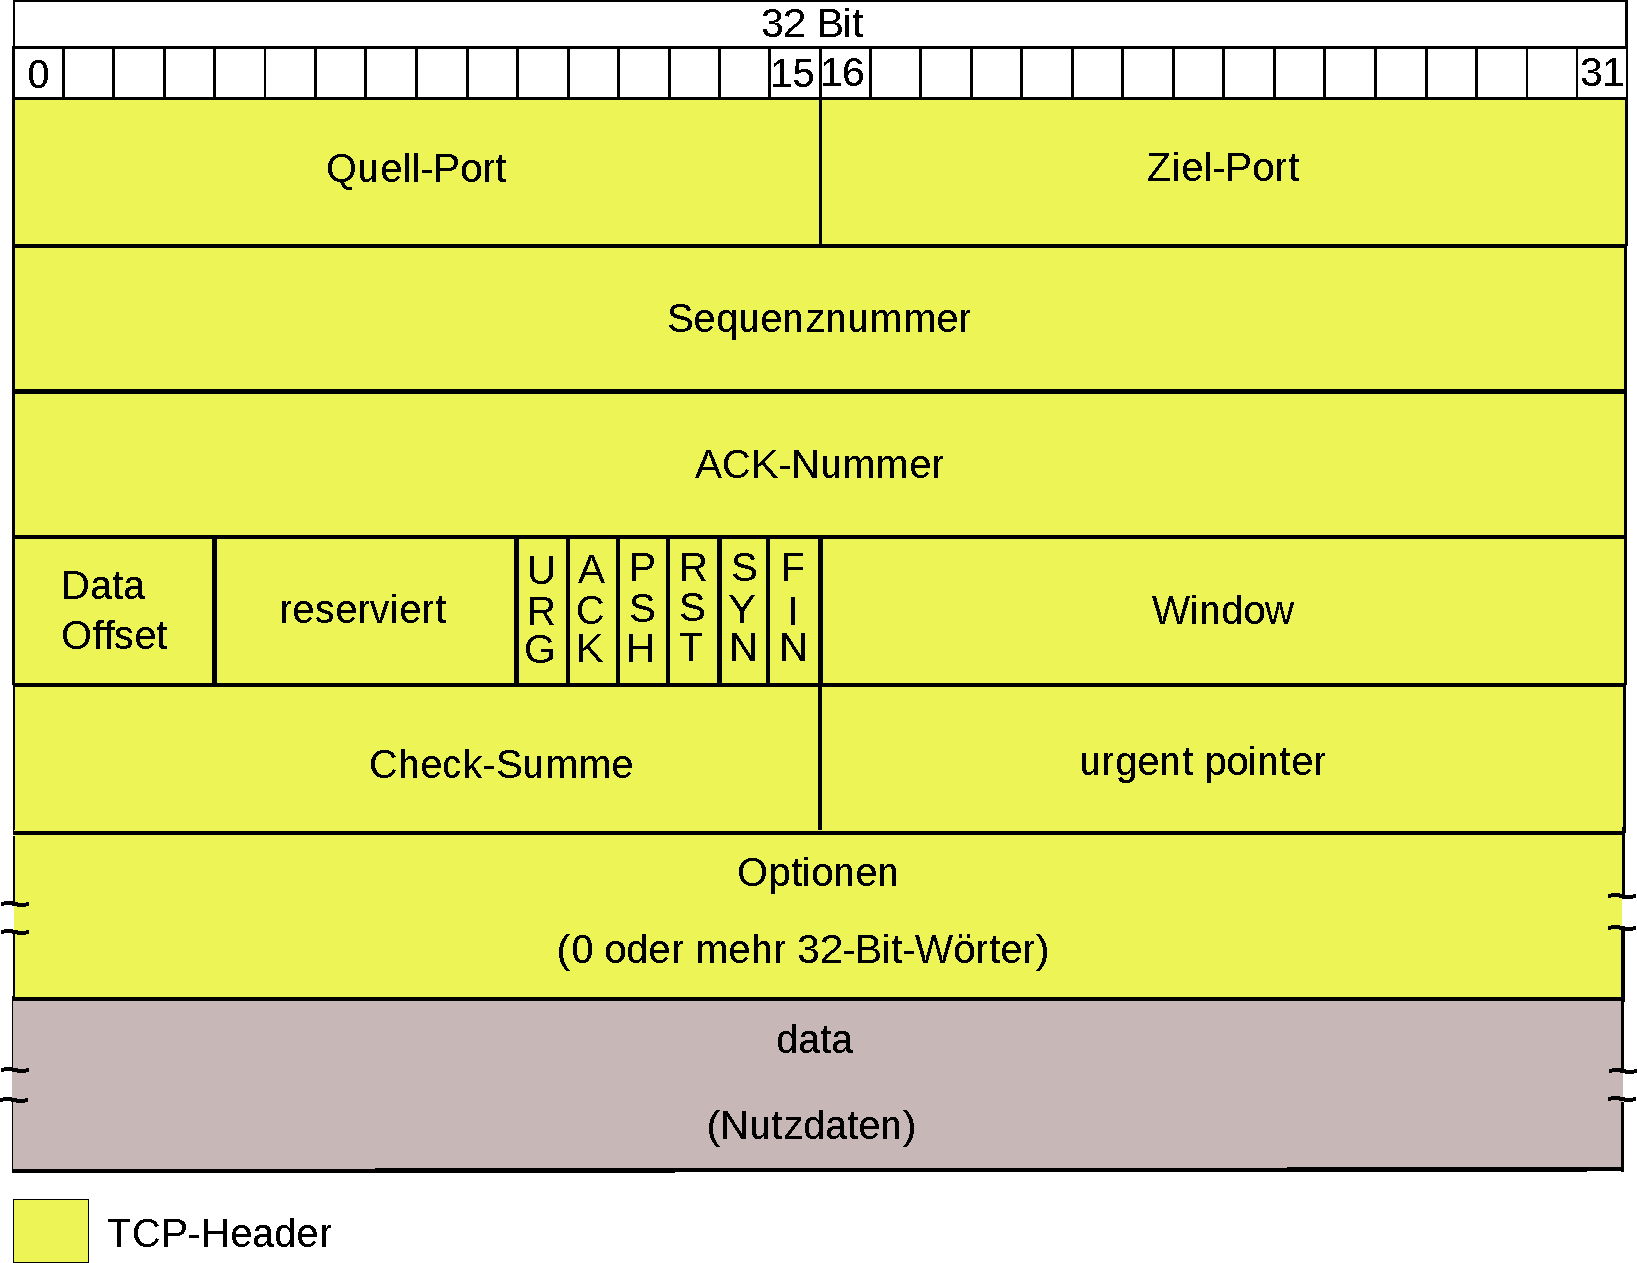
\includegraphics[width=0.5\textwidth]{tcpheader}
	\end{center} 
\end{frame}

\begin{frame}{TCP: Reliability and flow control}{}
	\begin{center} 
		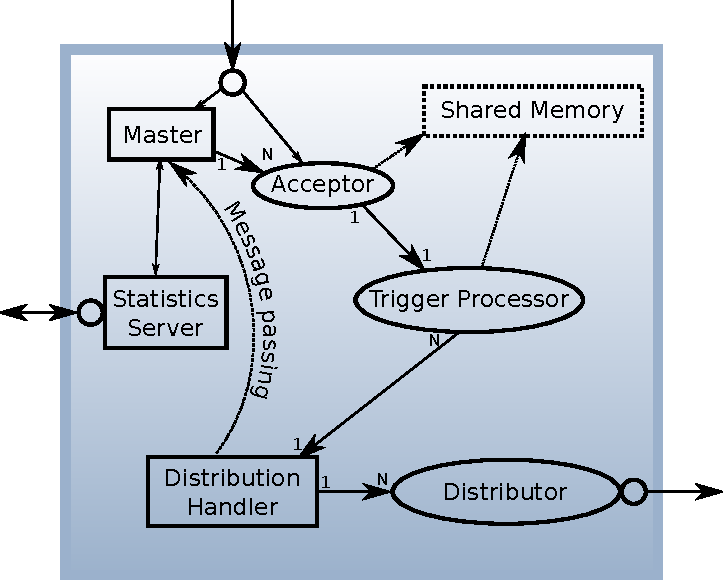
\includegraphics[height=0.7\textheight]{dataflow}
	\hspace{50}
		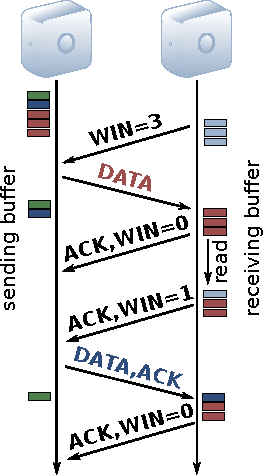
\includegraphics[height=0.7\textheight]{dataflowWindowSize}
	\end{center} 
\end{frame}

\begin{frame}{Congestion Avoidance}{}
	\begin{center} 
		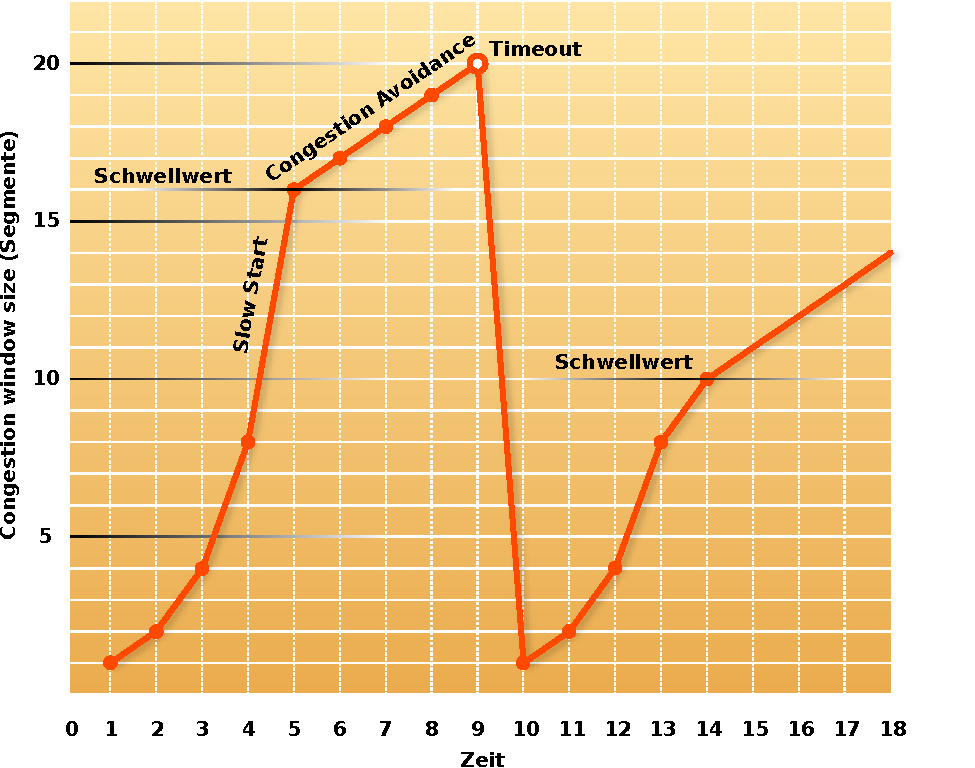
\includegraphics[width=0.8\textwidth]{slowStartundCongestionAvoidance}
	\end{center} 
\end{frame}

%\subsection{Performance tests}
\begin{frame}{Performance tests}{}
	\begin{block}{}
		\vspace{-0.35cm}
		\begin{ergo}
			TCP optimizes the usage of network resources
		\end{ergo}
	\end{block}
	\begin{alertblock}{But what does this cost? }
		Intuitionally one would guess: Higher CPU usage and longer latencies.
	\end{alertblock}
	but\ldots
\end{frame}

\begin{frame}{Data rate and CPU usage}{}
	\begin{center} 
		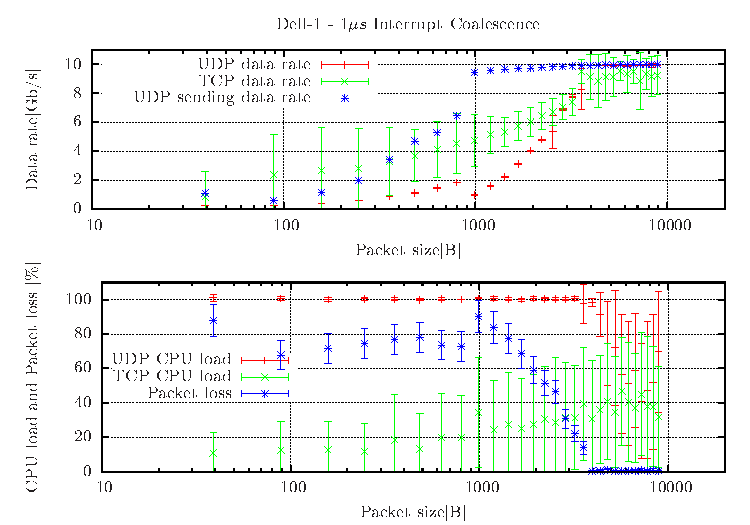
\includegraphics[width=0.9\textwidth]{proto_perf}
	\end{center} 
\end{frame}

\begin{frame}{TCP Offload Engine}{}
	\begin{block}{Network cards and drivers are optimized for TCP}
		\begin{itemize}
		  \item Checksumms and fragmentation calculated on hardware
		  \item Some drivers ignore interrupt coalescence of $0 \mu s$
		\end{itemize}
	\end{block}
	\begin{ergo}
		Using TCP reduces CPU usage $\Rightarrow$ more space for computation
	\end{ergo}
\end{frame}

\begin{frame}{Timing}{}
	\begin{center} 
		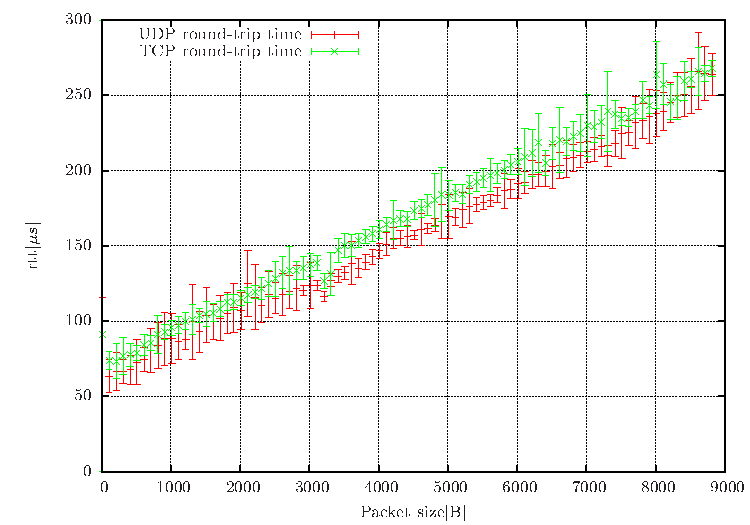
\includegraphics[width=\textwidth]{udp-tcp-rtt-eth0}
	\end{center} 
\end{frame}

\begin{frame}{Results}{}
	\begin{itemize}
	  \item TCP reduces CPU usage $\Rightarrow$ more space for computation
	  \item TCP has flow control and congestion avoidance	
	  \item TCP is reliable
	\end{itemize}
	
	\begin{alertblock}{TCP in FPGAs}
		TCP means high payload in hardware! \\
		$\Rightarrow$ TCP can only be used for PC to PC communication at NA62!
	\end{alertblock}
\end{frame}

\begin{frame}{TCP/UDP vs. basic IP}{}
	\begin{block}{Using standard interrupt/kernel based socket programming\ldots}
		\begin{itemize}
		  \item is optimized for TCP (drivers)
		  \pro is easy and many libraries can be used (e.g. boost::asio)
		  \contra induces high latency ($\approx 30-150 \mu s$)
		  \contra induces high packet loss??!!
		\end{itemize}
	\end{block}
	
	\begin{block}{Programming own Kernel modules\ldots}
		\begin{itemize}
		  \contra is hard stuff (only few small libraries)
		  \contra is bound to hardware
		  \pro highest performance possible
		\end{itemize}
	\end{block}
\end{frame}

	